
The goal of this chapter is ...

\section{Time on air}

\subsection{Regulations}

\subsection{Lab tests}

\begin{figure}[ht]
    \centering
    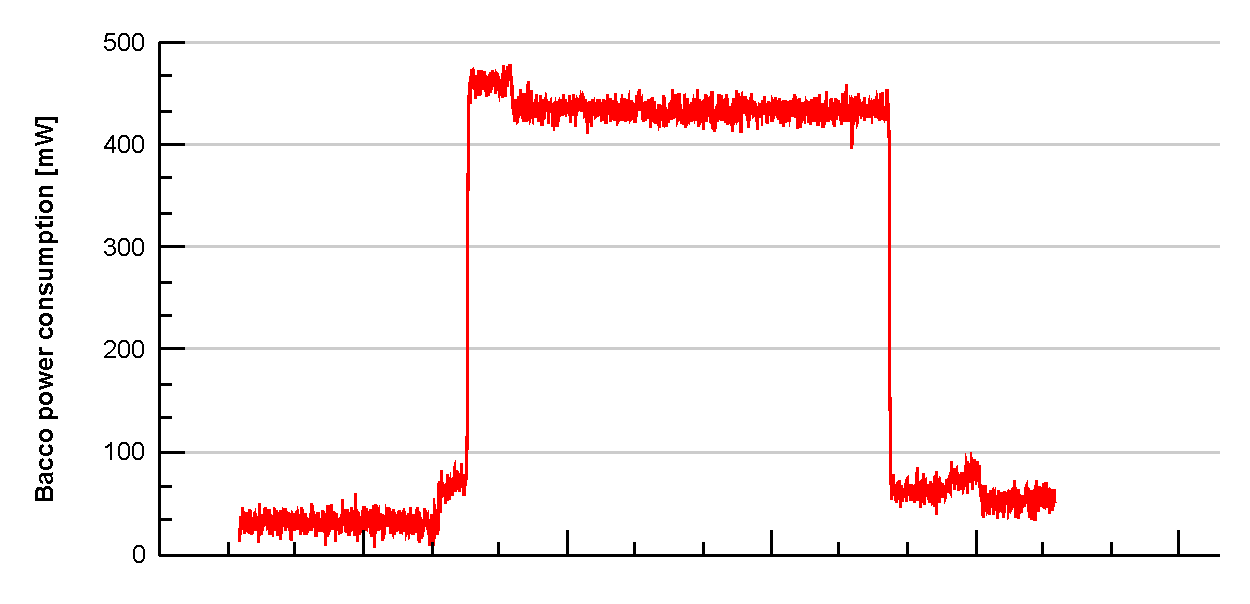
\includegraphics[width=1.0\textwidth]{images/bacco_SF7_14dbm_125khz_power.pdf}\\
    \vspace{-0.7cm}
    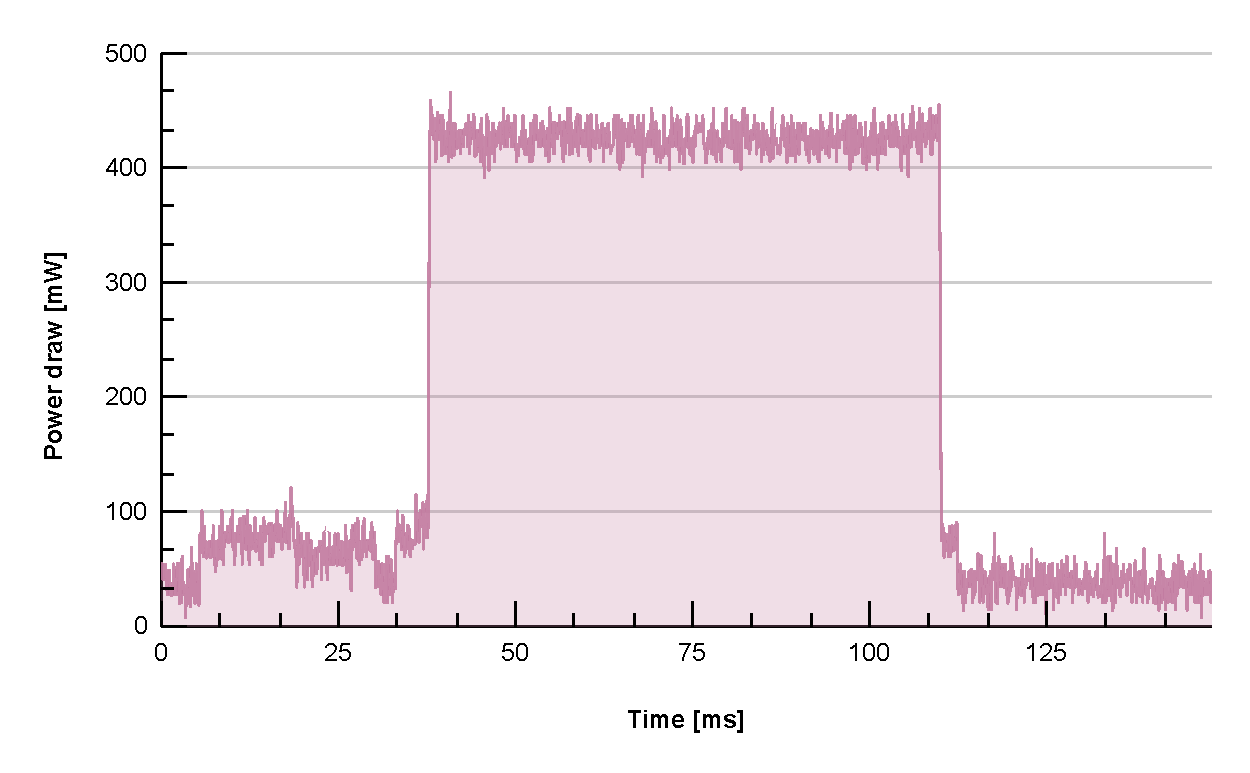
\includegraphics[width=1.0\textwidth]{images/lorawan_SF7_14dbm_125khz_power.pdf}
    \caption{Power draw of Bacco (in red) and LoRaWAN (in blue) during the transmission of a packet with a payload of 15
    bytes, using SF7, 14dBm, 125kHz bandwidth}
    \label{bacco SF7}
\end{figure}

Bacco:\\
delta time is 51.6ms and total energy is 21.3mJ
\\\\
LoRaWAN:\\
delta time is 71.8ms and total energy is 30.8mJ
